\section{Supplementary pooling and uncertainty analyses}
\label{sec:supplement}
The supplementary \meanmodel{} uses the same seed44, folds, observed-history protocol, future-state objective, and forecast classifier feature groups as \fullmodel{}, replacing spatial attention with mean pooling. It is reported separately from the three principal variants requested for the main analysis.
\begin{table}[t]
\centering
\caption{Supplementary pooling comparison using seed44. ForecastMean and ForecastAttention share forecast-based pCR readout and future-state supervision, and differ in spatial pooling.}
\label{tab:pooling}
\begin{tabular}{llrrr}
\toprule
Model & Landmark & AUROC & AP & F1 \\
\midrule
ForecastMean & T0 & 0.7317 & 0.5812 & 0.5446 \\
ForecastMean & T1 & 0.7367 & 0.5869 & 0.5523 \\
ForecastMean & T2 & 0.7361 & 0.5856 & 0.5405 \\
ForecastMean & Macro & 0.7348 & 0.5845 & 0.5458 \\
\midrule
ForecastAttention & T0 & 0.7294 & 0.5924 & 0.5334 \\
ForecastAttention & T1 & 0.7381 & 0.6012 & 0.5563 \\
ForecastAttention & T2 & 0.7421 & 0.6033 & 0.5510 \\
ForecastAttention & Macro & 0.7365 & 0.5990 & 0.5469 \\
\bottomrule
\end{tabular}
\end{table}

\begin{table}[t]
\centering
\caption{Exploratory paired patient-bootstrap intervals for three-landmark mean differences (2,000 shared patient resamples). Intervals condition on the fixed seed44 models; they exclude retraining and seed-selection uncertainty.}
\label{tab:bootstrap}
\small
\begin{tabular}{llr}
\toprule
Comparison & Metric & Difference [95\% interval] \\
\midrule
DirectReadout -- NoJEPA & AUROC & +0.0084 [-0.0051, +0.0219] \\
DirectReadout -- NoJEPA & AP & +0.0097 [-0.0128, +0.0315] \\
DirectReadout -- NoJEPA & F1 & +0.0102 [-0.0118, +0.0325] \\
ForecastAttention -- NoJEPA & AUROC & +0.0146 [-0.0062, +0.0369] \\
ForecastAttention -- NoJEPA & AP & +0.0198 [-0.0161, +0.0597] \\
ForecastAttention -- NoJEPA & F1 & +0.0032 [-0.0339, +0.0398] \\
ForecastAttention -- DirectReadout & AUROC & +0.0062 [-0.0129, +0.0268] \\
ForecastAttention -- DirectReadout & AP & +0.0101 [-0.0244, +0.0482] \\
ForecastAttention -- DirectReadout & F1 & -0.0070 [-0.0396, +0.0237] \\
\bottomrule
\end{tabular}
\end{table}

\begin{figure}[t]
\centering
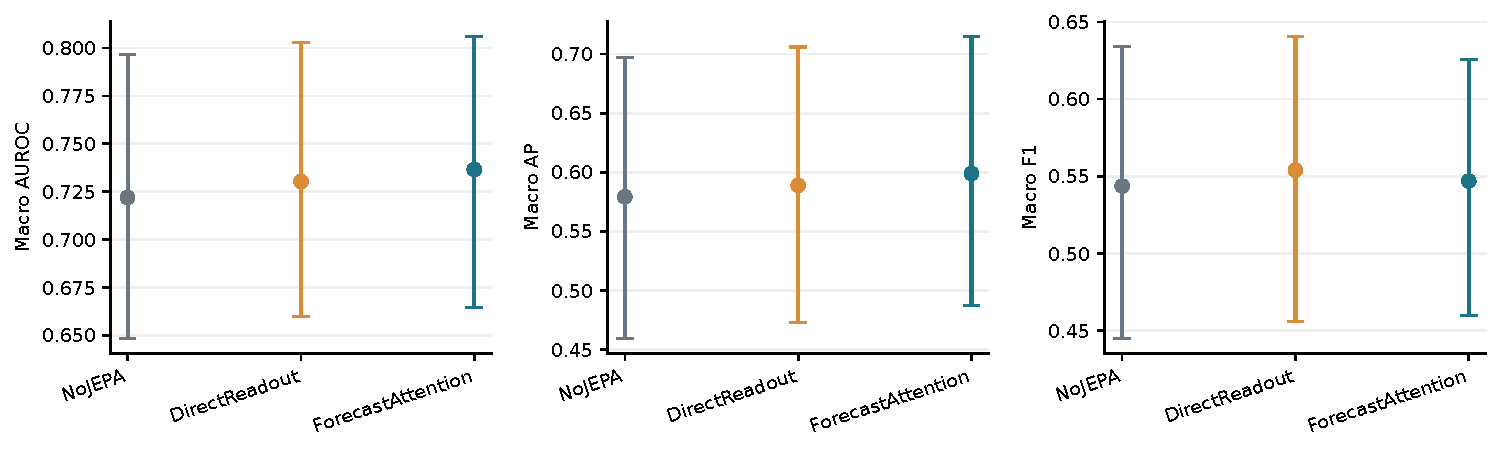
\includegraphics[width=\textwidth]{figures/patient_bootstrap.pdf}
\caption{Three-landmark mean metrics with exploratory 95\% percentile patient-bootstrap intervals. All 2,000 resamples preserve pairing across models, folds, and landmarks. Intervals describe patient-sampling uncertainty conditional on the trained seed44 models and do not account for seed selection or retraining.}
\label{fig:bootstrap}
\end{figure}
\section{Reproducibility and reporting items to complete}
The accompanying source package includes aggregate result CSV files, source-report hashes, the bootstrap procedure, figure-generation code, and a build script. It does not include patient identifiers, patient-level prediction rows, MRI volumes, or model checkpoints. All four model variants in this package use training seed44; the bootstrap random-number seed controls patient resampling only.

\todo{Before submission, complete the author and ethics statements; verify the pCR endpoint and visit timing; document codec and segmentation training-patient provenance; add matched external baselines and the locked multi-seed sensitivity analysis; audit external-cohort independence; and confirm the journal's current submission and anonymization requirements.}
